\chapter{气体动理论}
\section{选择题}
\exercise B

\solve 微观上,气体温度表示气体分子的运动速度,对于单个或少数分子,温度的概念失去了意义。宏观上,气体的温度表示气体分子的平均冷热程度。

\exercise B

\solve
由$v_p=\sqrt{\frac{2kT}{u}}$,$u\left(\ce{O2}\right)>u\left(\ce{H2}\right)$,$v_p\left(\ce{O2}\right)<v_p\left(\ce{H2}\right)$,故a表示氧气分子的速率分布曲线。

由于$k$为常量,$T$相同,
$\frac{v_p\left(\ce{O2}\right)}{v_p\left(\ce{H2}\right)}=\sqrt{\frac{2kT/32}{2kT/2}}=\frac{1}{4}$

\exercise C

\solve 自由度为$i$的分子的平均动能为$ikT/2$。

\exercise A

\solve
由$
\sqrt{\overline{v^2}\ }=\sqrt{\frac{3kT}{u}}$,
因为$u\left(\ce{H2}\right)> u\left(\ce{H2}\right)$,且
$\sqrt {\overline{v^2}\left(\ce{O2}\right)} = \sqrt {\overline{v^2}\left(\ce{H2}\right)}$,故
$T\left(\ce{O2}\right)>T\left(\ce{H2}\right) $

\exercise B

\solve 等温过程系统内能不变。

\exercise A

\solve
已知
$\varepsilon_{\ce{He}}=\varepsilon_{\ce{N2}},n_{\ce{He}}=n_{\ce{N2}}$

由$p=\frac{2}{3}n\overline{\varepsilon}$可知$p_{\ce{He}}=p_{\ce{N2}}$,由$\overline{\varepsilon}=\frac{3}{2}kT$可知$T_{\ce{He}}=T_{\ce{N2}}$

\exercise A

\solve
$p V = \nu R T= \frac { m } { M } R T \Rightarrow p M= \rho R T \Rightarrow \rho= \frac { p M } { R T }$

由于水滴静止,则$p_{\ce{H2}} =p_{\ce{O2}}$

又因为T相同,则

$$
\frac {\rho_{\ce{H2}} } {\rho_{\ce{O2}} } = \frac{pM_{\ce{H2}}/RT} {pM_{\ce{O2}}/RT}=\frac{1}{16}
$$

\exercise D

\solve
由$
 \overline { z } = \sqrt { 2 } \pi d ^ 2 \overline { v } n,\lambda = \frac { 1 } { \sqrt { 2 } \pi d ^ { 2 } n } $,代入$n = \frac { p } { k T }$,得$\overline{ z } = \sqrt { 2 } \pi d ^ { 2 } \overline { v } \frac { p } { k T }$

$\because\ T$不变,$\overline{v}$不变;而$p$变为原来的两倍

$\therefore\ z^{\prime} = 2\overline{z}$

又$\because\ \overline{v}=\overline{\lambda}\overline{z}$,$\therefore\ \lambda ^ { \prime } = 2 \overline{ \lambda }$

\exercise C

\solve

$2\ce{H2O}\ce{->}2\ce{H2}+\ce{O2}$

气体内能$E=\frac{i}{2}\nu RT$。对于刚性分子,双原子分子气体的$i=5$,多原子分子气体的$i=6$,则

$E _ { 0 } = 2 \cdot \frac { 6 } { 2 } R T$

$E_0^ { \prime }=2\cdot\frac{5}{2}R T + \frac { 5 } { 2 } R T = \frac { 15 } { 2 } R T$

$\therefore \frac { 15 } { 2 } R T \div 6 R T = 125 \%$

\exercise B

\solve
由$ 
\sqrt{\overline{z}\ }= \sqrt { \frac { 3 k T } { u } }$,$T _ { 2 }= \frac { 3 } { 2 } T _ { 1 }$得:

$T _ { 2 } = \left( \frac { 3 } { 2 } \right) ^ { 2 } T _ { 1 }= 280 \times \frac { 9 } { 4 } = 630 $K

\section{填空题}
\exercise 
$\int _ { v _ 1} ^ { v _2 } f ( v ) N\di{v}$
\qquad
$\frac { \int _ { v _ { 1 } } ^ { v _ { 2 } } v f ( v )\di{v}} { \int _ { v _ { 1 } } ^ { v _ { 2 } } f ( v )\di{v}}$
\qquad
$N \cdot \frac { 1 } { 2 } m \int _{v_1}^{v_ 2} v^2f( v )\di{v}$

\solve
(1)

$$
\begin{aligned}
\frac {\di{N}} { N } & = f ( v )\di{v}\\
\di{N}& = N f ( v )\di{v}\\
N ^ { \prime } = &\int\di{N}= \int _ { v_1 } ^ { v _ { 2 } } N f ( v )\di{v}
\end{aligned}
$$

(2)
$$
\begin{aligned}
v_1 \sim v_2 \mbox{的平均速度}&=\frac{\mbox{这个区间里每个分子速度之和}}{\mbox{这个区间里分子总数}}\\
&=\dfrac { \int _ { v _ { 1 } } ^ { v _ { 2 } } v\di{N}} { \int _ { v _ { 1 } } ^ { v _ { 2 } }\di{N}} = \dfrac { N \int _ { v _ { 1 } } ^ { v _ { 2 } } v f ( v )\di{v}} { N \int _ { v _ { 1 } } ^ { v _ { 2 } } f ( v )\di{v}} \\
&=\dfrac { \int _ { v _ {1 } } ^ { v _ { 2 } } v f ( v )\di{v}} { \int _ { v _ { 1 } } ^ { v _ { 2 } } f ( v )\di{v}}
\end{aligned}
$$

(3)
$$
\begin{aligned}
\mbox{总平动动能之和}&=\mbox{每个分子平动动能之和}\\&= \int _ { v _ { 1 } } ^ { v _ { 2 } } \frac { 1 } { 2 } m v ^ { 2 }\di{N}\\
&=\dfrac{1}{2}m N \int _ { v _ { 1 } } ^ { v _ { 2 } } v ^ { 2 } f ( v )\di{v}
\end{aligned}
$$

\exercise $\frac { N _ { A } } { N _ { A } + N _ { B } } f _ { A } ( v ) + \frac { N _ { B } } { N _ { A } + N _ { B } } f _ { B } ( v )$

\solve $\frac{N_A}{N_A+N_B}$指的是A在混合气体里占比,B同理。由概率论知识可知,对概率密度求加权平均即得结果。

\exercise
$n _ { 0 } e ^ { - \frac { m g z } { k T } } \qquad z = - \frac { k T \ln ^ { \frac { p } { p_0 } } } { m g }$

\solve 由玻尔兹曼分布律:$
n = n _ { 0 } e ^ { - \frac { m g z } { k T } }$

$p= p _ { 0 } e ^ { - \frac { m g z } { k T } }$,故$z= - \frac{kT\ln\frac{p}{p_0}}{ m g }$

\exercise 升高\qquad 升高

\solve (1)温度应上升。因为高速运动的氧气瓶中的分子是在杂乱无章运动的基础上附加上x方向定向运动速度。氧气瓶静止下来后,气体分子与氧气瓶发生碰撞,高速的x方向定向运动动能通过分子之间的频繁碰撞逐步平均分配到y、z方向的热运动动能上去,所以温度上升。

(2)$pV=\nu RT$,$T$增大,$V,\nu,R$都不变,所以$p$增大。

\exercise $\frac{3kT}{2}$\qquad 温度是大量分子热运动的集体表现,对单个或少数分子来说,温度的概念就失去了意义。

\exercise $7.82 \times 10 ^ { 7 } s ^ { - 1 } \qquad5 \times 10 ^ { - 5 } \mathrm { cm }$

\solve
由$\bar { \lambda } = \frac { k T } { \sqrt { 2 } \pi d^2p }$,$\bar { \lambda } $和$\bar { v } $成反比.

$p _0= 1 \times 10 ^ { 5 }\mathrm{Pa}$

$p _1= 1 \times 10 ^ { 4 }\mathrm{Pa}$

${ \therefore\ \overline{\lambda^{\prime} } = 10 \bar { \lambda } = 5 \times 10 ^ { - 5 }\mathrm{ cm }}$

${ z ^{\prime } = \frac { 1 } { 10 } \bar { z } = 7.82 \times 10 ^ { 7 }\mathrm{s^{-1}}}$

\exercise 1:4:16\qquad 1:2:4

\solve
$\sqrt {\overline{ v^2}} = 1.73 \sqrt { \frac { R T } { M } }$

$\because \sqrt{\overline{v_A^2}}:\sqrt{\overline{v_B^2}}:\sqrt{\overline{v_C^2}}= 1 : 2 : 4$

$\therefore T _A: T _B: T _C= 1 : 2 ^2: 4 ^2= 1 : 4 : 16 $

$n = \frac { N } { V } = \frac { \nu N _ { A } } { V }$

$\therefore n \propto \frac { \nu } { V }$

$\therefore \frac { \nu _1} { V _1} : \frac { \nu _2} { V _2} : \frac { \nu _3} { V _3}  = n _1: n _2: n _3= 4 : 2 : 1 $

由$p V  = \nu R T$,$p = \frac { \nu R T } { V }  = \frac { \nu } { V } \cdot T \cdot R $

$\therefore p  \propto \frac { \nu } { V } T$

$ \therefore p _1: p _2: p _3= 4 \times 1 : 2 \times 4 : 1 \times 16 = 1 : 2 : 4  $

\exercise 6

\solve (1)刚性多原子分子(甲烷)共有6个自由度。

(2)由于分子热运动的无规则性,任何一种运动都不比其他运动占有特别的优越性,所以机会相等,所以分子绕其质心转动对$i$的贡献为3.

\exercise $\geqslant 0 $\qquad 不变 \qquad 增

\solve
(1)孤立系统的熵永远也不会减少。

(2)可逆过程熵不变。

(3)由于ΔS$\geqslant 0$,不可逆过程熵增。


\exercise 0 \qquad 增

\solve(1)气体自由膨胀,对外界不做功(A=0)。绝热过程Q=0,ΔE=-A=0。故内能增量为0。

(2)孤立系统的熵永远也不会减少。


\section{计算题}
\exercise

\solve
(1)
%\begin{figure}[!ht]
%	\centering
%	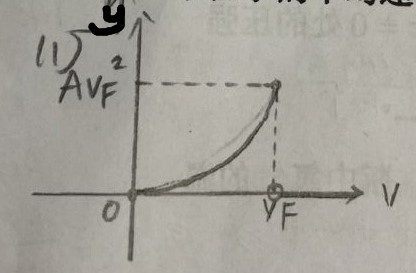
\includegraphics[width=0.35\textwidth]{Chp12_21.jpg}
%\end{figure}
\begin{figure}[!h]
	\centering
	\begin{tikzpicture}[scale=1.2]
	%坐标轴和点
	\draw (0,0) node[below left] {$O$};
	\draw [->] (-0.5,0) -- (3,0) node[right] {$v$};
	\draw [->] (0,-0.5) -- (0,3) node[right] {y};	
	\draw (2,-0.05) -- (2,0.05)
	node[below,outer sep=4pt,fill=white,font=\small]
	{$v_F$} (2,0);	
	\draw (-0.05,2) -- (0.05,2)
	node[left,outer sep=3pt,fill=white,font=\small]
	at (0,{2}) {$Av_F^2$};	
	%线
	\draw [dashed,-] (0,2) -- (2,2);
	\draw [dashed,-] (2,0) -- (2,2);
	\draw [-,domain=0:2,smooth] plot(\x,{0.5*\x*\x});
	\end{tikzpicture}
\end{figure}

(2)
\begin{align*}
\int _ { 0 } ^ {+\infty}f(v)\di{v}
&=\int _ { 0 } ^ {v_F}Av^2\di{v}\\
&=\left. \dfrac { 1 } { 3 } A v ^ { 3 } \right| _ { 0 } ^ { v _ { F } }\\
&=\dfrac { 1 } { 3 } A v_F^3= 1 \\ 
A&=\dfrac{3}{ v_F^3 }
\end{align*}

(3)
与速率分布函数极大值所对应的速率称为最概然速率。

\therefore $v_P=v_F$

(4)
\begin{gather*}
{\overline{ v } = \int _ { 0 } ^ { v _ { F } } v f ( v )\di{v}} \\
 {\overline{ v } = \int _ { 0 } ^ { v _ { F } } v \cdot \frac { 3 } { v _ { F } ^ { 3 } } v ^ { 2 } d v = \left. \frac { 3 } { 4 v _ { F } ^ { 3 } } v ^ { 4 } \right| _ { 0 } ^ { v _ { F } } = \frac { 3 } { 4 } v _ { F } } 
\end{gather*}

(5)
\begin{gather*}
 {\overline{ v } = \int _ { 0 } ^ { v _F} v f ( v )\di{v}} \\
{\overline{ v } = \int _ { 0 } ^ { v _ { F } } v \cdot \frac { 3 } { v _ { F } ^ { 3 } } v ^ { 2 } d v = \left. \frac { 3 } { 4 v _ { F } ^ { 3 } } v ^ { 4 } \right| _ { 0 } ^ { v _ { F } } = \frac { 3 } { 4 } v _ { F } } \\
{\overline{ v } ^ { \prime } = \int _ { \frac { v _ { F } } { 2 } } ^ { v _ { F } } \frac { 3 } { v _ { F } ^ { 3 } } v ^ { 3 } d v = \left. \frac { 3 } { 4 v _ { F } ^ { 3 } } v ^ { 4 } \right| _ { \frac { v _ { F } } { 2 } } ^ { v _ { F } } = \frac { 3 } { 4 v _ { F } ^ { 3 } } \left( v _ { F } ^ { 4 } - \frac { 1 } { 16 } v _F^4\right) = \frac { 45 } { 64 } v _F}
\end{gather*}

\exercise

\solve
(1)
由$p = n k T$
\begin{gather*}
n = \frac { p } { k T } = 2.415 \times 10 ^ { 25 } \\ 
n ^ { \prime } = 2.415 \times 10 ^ { 16 }
\end{gather*}
$\therefore N=2.415\times 10^{16}\mbox{(个)}$

(2)
$$
m_0= \frac { M } {N_A} = 5.31 \times 10 ^{-23}\mathrm{g}
$$

(3)
\begin{align*}
\rho &= \frac {m} { V } = \frac {Nm_0}{V}\\
&= \frac { 2.415 \times 10 ^ { 16 } \times 5.31 \times 10 ^ { - 23 } } { 10 ^ { - 9 } } \times 10 ^ { - 3 } \\
&= 1.28236 \times 10^{27}\mathrm{kg/m^3}
\end{align*}

(4)
$$
\overline{ v } = \sqrt { \frac { 8 k T } { \pi m _ { 0 } } } = \sqrt { \frac { 8 \times 1.38 \times 10 ^ { - 23 } \times 300 } { \pi \times 5.31 \times 10 ^ { - 23 } \times 10 ^ { - 3 } } } = 446 \mathrm { m } / \mathrm {s}
$$

\exercise

\solve
(1)
\begin{align*}
p &= p _ { 0 } e ^ { - \frac { \mu g h } { k T } } = p _ { 0 } e ^ { - \frac { M g h } { R T } } \\
&= 0.633 p _ { 0 } \\
&= 6.45 \times 10 ^4\mathrm{Pa}
\end{align*}
(2)
每口吸入的空气体积$V$不随海拔变化而变化。相同质量即$n$相同。

忽略气温随高度变化时,T为定值。由$pV=nRT$
\[
p_{0}\cdot 17 V =0.633p_0 \cdot x V
\]

$x = 26.7$,故$x$取27. 

\exercise

\solve
(1)
\begin{gather*}
{ \rho = \frac { m } { V } = \frac { \nu m _ { 0 } } { V } = 11.3\mathrm{g /cm^3} } \\
p V = \nu R T\\
\dfrac { \nu } { V } = \frac { p } { R T } = \dfrac { 1.01 \times 10 ^ { 3 } } { 8.314 \times 300 } = 0.405\\
m _ { 0 } = \rho \frac { V } { \nu } = \frac { 11.3 } { 0.405 } = 27.9012 \approx 28
\end{gather*}

则可能是\ce{N2},\ce{CO},\ce{CH2=CH2}等。

(2)
$$
\sqrt{\overline{v^{2}}}=\sqrt {\frac{3kT}{\mu}}=1.73\sqrt {\frac{RT}{M}}=1.73\times\sqrt{\frac{8.314\times 300}{28\times10^{-3}}}=516.8\mathrm{m}/\mathrm{s}
$$

(3)
\begin{align*}
\overline{\varepsilon}_{\mbox{\tiny 平}}&=\frac{3}{2}kT\\
&=\frac{3}{2}\times 1.38\times 10^{-23}\times 300\\
&=6.21\times 10^{-21}\\
\overline{\varepsilon}_{\mbox{\tiny 转}}&=kT\\
&=4.14\times 10^{-21}
\end{align*}

(4)单位体积总平动动能=1个分子平均平动动能$\times$分子数密度,故

$$E_{\mbox{\tiny 平总}}=\overline{ \varepsilon } _ {\mbox{\tiny 平}}n=\overline{ \varepsilon } _ {\mbox{\tiny 平}}\frac{p}{kT}=6.21 \times 10^{-21} \times \frac { 1.01 \times 10 ^3} { 1.38 \times 10 ^ { - 23 } \times 300 } = 1515\mathrm{J}$$

同理,$\overline{ \varepsilon}_{\mbox{\tiny 转总}}=1010\mathrm{J}$

(5)
$$
E = \nu \frac{i}{2}RT=0.3 \times \frac { 5 } { 2 } \times 8.314 \times 300 = 1870.65\mathrm{J}
$$